\documentclass{beamer}
\usepackage{algorithm}
\usepackage{algorithmic}
\usepackage{listings}

\DeclareMathOperator*{\argmin}{arg\,min}
\usepackage{amsmath}
\usepackage{graphicx}
\newcommand{\mas}{\text{\normalfont mas}}

\usetheme{metropolis}          
\title{Bandit Problems}
\date{\today}
\author{Vishakh Gopu, Frederik Jensen}
\institute{Advanced Machine Learning - Spring 2017}
\begin{document}
\maketitle

%%%%%%%%%%%%%%%%%%%%%%%%%%%%%%%%%%%%%%%%%%%%%%%%%%%%%%% 
% Introduction
%%%%%%%%%%%%%%%%%%%%%%%%%%%%%%%%%%%%%%%%%%%%%%%%%%%%%%% 

\section{Introduction}
\begin{frame}{Overview of Papers}   
  Three main problem settings: 
  \begin{enumerate}
  \item
    Restless Bandits
    \begin{itemize}
    \item
      Bertsimas, Dimitris, Nin\~o-Mora, Jos\'e. 2000. Restless Bandits, Linear Programming
      Relaxations, and a Primal-Dual Index Heuristic. Operations Research, 48(1), 80–90.
    \end{itemize}
  \item
    Graph Structured Feedback
    \begin{itemize}
    \item
      Alon, Noga, Cesa-Bianchi, Nicol\`o, Gentile, Claudio, Mannor, Shie, Mansour, Yishay,
      Shamir, Ohad. 2014. Nonstochastic Multi-Armed Bandits with Graph-Structured Feedback.
      CoRR, abs/1409.8428.
    \end{itemize}
  \item
    Handling Variance in Rewards
    \begin{itemize}
    \item
      Hazan, Elad, Kale, Satyen. 2009. Better Algorithms for Benign Bandits. Pages 38–47 of: 
      Proceedings of the Twentieth Annual ACM-SIAM Symposium on Discrete Algorithms. SODA '09.
      Philadelphia, PA, USA: Society for Industrial and Applied Mathematics.
    \end{itemize}
  \end{enumerate}
\end{frame}

\begin{frame}{Outline}
  \begin{enumerate}
  \item
    Graph Structured Feedback Review
  \item
    Better Algorithms for Benign Bandits Review
  \item
    Exploration and future work
    
  \end{enumerate}
\end{frame}


% \section{Problem Definition}
% \begin{frame}
%   \begin{enumerate}
%     \item Online learner
%     \item At each round $t$, picks an action from $i\in\mathcal{K}$
%     \item Loss $L$ only disclosed for action $i$
%     \item Regret guarantees
%   \end{enumerate}
% \end{frame}


\section{Non-Stochastic Bandits with Graph Structured Feedback}
%%%%%%%%%%%%%%%%%%%%%%%%%%%%%%%%%%%%%%%%%%%%%%%%%%%%%%% 
% Non stochastic bandits with graph structured feedback
%%%%%%%%%%%%%%%%%%%%%%%%%%%%%%%%%%%%%%%%%%%%%%%%%%%%%%% 
\begin{frame}{Problem Reformulation}
  \begin{itemize}
    % Details about the problem.
    \item Web advertisement example

    % How is it different from the general bandit
    \item Partial information setting

    \item Action set $\mathcal{K}\in \mathbb{R}^n$ for $n$ experts
    \item Feedback graph $G_t(\mathcal{K}, D_t)$ 
    \begin{enumerate}
      \item Edge $(i,j)\in D_t$ if playing $i$ at time $t$ reveals loss $j$
      \item Write $i\overset{t}{\to}j$
    \end{enumerate}
  \end{itemize}
  % setting.
 % Motivate by example of web advertisement.    
\end{frame}

\begin{frame}{High Level Overview}
  \begin{itemize}
    \item Modification of Exp3 based on maximum acyclic graph $\mas(G_t)$ and the independence number $\alpha(G_t)$
    \item Scenarios
      \begin{figure}[]
      \center
      \begin{tabular}{ | c | c | c | }
          \hline
          \textbf{Algorithms} & \textbf{Uninformed} & \textbf{Informed} \\
          \hline
          \textbf{Directed} & Exp3-SET ($\mas{G_t}$) & Exp3-DOM\\
          \hline
          \textbf{Undirected} & Exp3-SET ($\alpha(G_t)$) & Exp3-DOM\\
          \hline
      \end{tabular}
      \end{figure}
    \item $\mas(G_t) \geq \alpha(G_t)$
  \end{itemize}
  % Conceptual understanding - interpolation between
  % different settings (similar to the bonus problem) - plug in and get results.
\end{frame} 

\begin{frame}{Guarantees of Exp3-SET}
  \begin{itemize}
    \item Key quantity: $$Q_t=\sum_{i\in |\mathcal{K}|}\frac{p_{i,t}}{q_{i,t}} = \sum_{i\in |\mathcal{K}|}\frac{p_{i,t}}{\sum_{j:j\overset{t}{\to}i} p_{j,t}}$$

    \item The regret of Exp3-SET satisfies
    $$
    R_t\leq \frac{\ln |\mathcal{K}|}{\eta} + \frac{\eta}{2}\sum_{t=1}^T\mathbb{E}[Q_t].
    $$
   
    \item Interpolation

 \end{itemize}
\end{frame}

\begin{frame}{Guarantees of Exp3-SET (2)}
\begin{itemize}
    \item For Exp3-SET, let $\mas(G_t)\leq m_t$ for $t=1,...,T$. Then, setting $\eta=\sqrt{(2\ln |\mathcal{K}|)/\sum_{t=1}^T m_t}$ yields the regret bound: $$R_T\leq \sqrt{2(\ln |\mathcal{K}|)\sum_{t=1}^Tm_t}$$

     \item Problem: Loose bound, computing $\mas(G_t)$ and $\alpha(G_t)$ (NP-hard) 
\end{itemize}
\end{frame}

\begin{frame}{Loose regret bound for Exp3-SET}
  \begin{itemize}
   \item Counter example for $|\mathcal{K}|=4$

   \begin{figure}
    \centering
    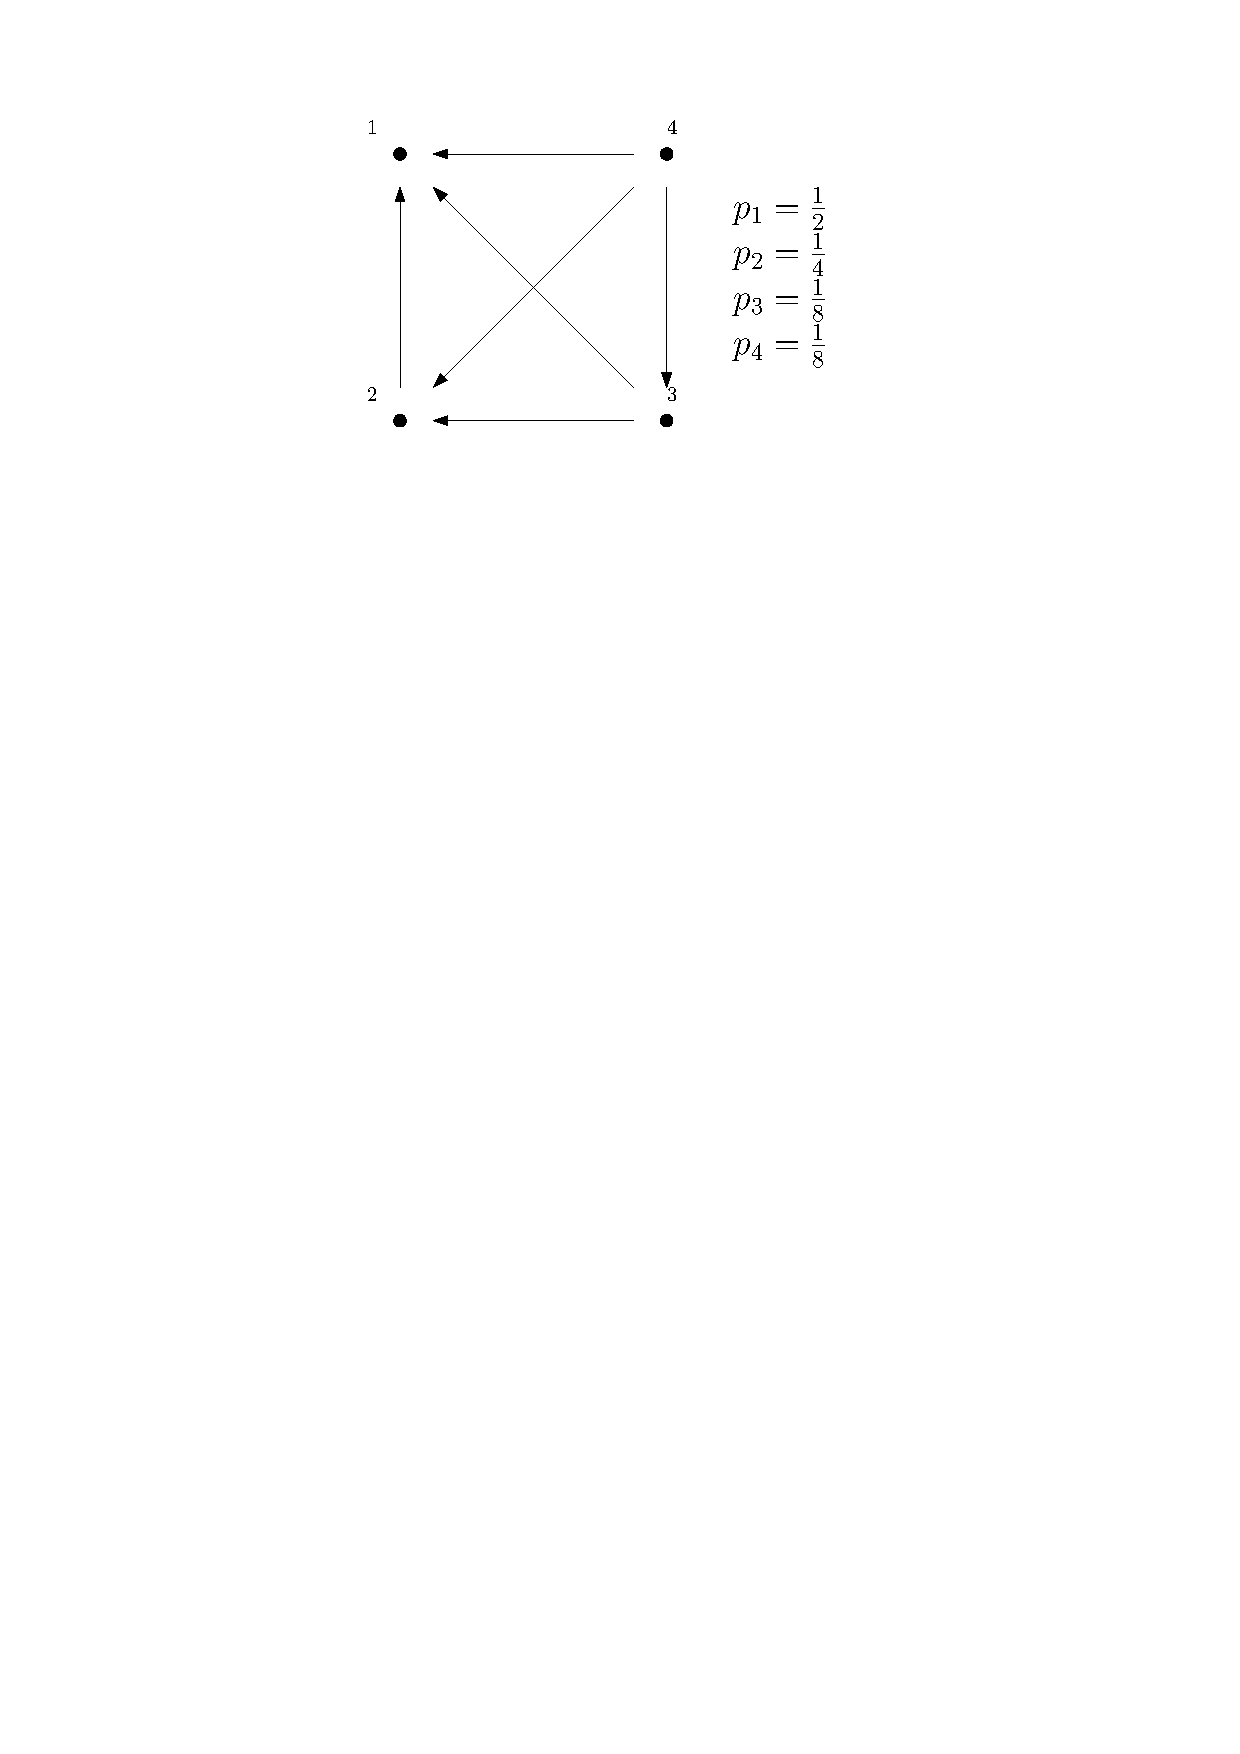
\includegraphics[scale=0.7]{dag}
   \end{figure}


   \item $Q=\sum_{i=1}^{|\mathcal{K}|}\frac{p_i}{p_i+\sum_{j:j\to i}p_j}=\sum_{i=1}^{|\mathcal{K}|}\frac{p_i}{\sum_{j=i}^{|\mathcal{K}|}p_j}=\frac{K+1}{2}$

   \item Tighter bounds $\to$ Exp3-DOM
  \end{itemize}
\end{frame}

\begin{frame}{Exp3-DOM}
  \begin{itemize}
    \item Runs $\log |\mathcal{K}|$ variants of Exp3 with explicit exploration
    \item Picks result based on size of the dominating set, $R_t$
    \item $R_t$ computed with Greedy Set Cover algorithm 
    \item Using the doubling trick, the regret of Exp3-DOM satisfies 
      $$R_T\leq \mathcal{O}\Bigg(\ln(|\mathcal{K}|)\sqrt{(\ln |\mathcal{K}|T)\sum_{t=1}^T\alpha(G_t)}+\ln(|\mathcal{K}|)\ln (|\mathcal{K}|T)\Bigg)$$
  \end{itemize}
\end{frame}

\section{Better algorithms for benign bandits}
%%%%%%%%%%%%%%%%%%%%%%%%%%%%%%%%%%%%%%%%%%%%%%%%%%%%%%% 
% Total variation
%%%%%%%%%%%%%%%%%%%%%%%%%%%%%%%%%%%%%%%%%%%%%%%%%%%%%%% 
\begin{frame}{High level overview}

  \begin{enumerate}
  \item
    Losses might not be truly adversarial
    \begin{itemize}   
    \item
      Example: planning a route to work in traffic
    \end{itemize}
    \item
      Can we take advantage of low variation in our algorithm?
    \item
       Can we bound regret based on variability?
      \begin{itemize}
        \item
          Learning should depend on the \textit{total variation} of the losses
        \end{itemize}
  \end{enumerate}
\end{frame}

\begin{frame}{Problem description}
  \begin{enumerate}
    \item
    Online bandit convex optimization
    \begin{itemize}
      \item
        Adversarial but oblivious
      \item
        Point ${\bf x}_t$ from $\mathcal{K}$, compact set
      \item
        Cost vector $f_{t}$
      \end{itemize}
    \item
      Take the total variation
      $Q_T=\sum_{t=1}^T \| f_t - \mu \|^2$
    \item
      Recall barrier functions and self concordant functions
      \begin{itemize}
        \item
          Ensure that we always sample from the feasible set
        \end{itemize}
     \item
       FTRL ++
        \begin{align*}
          \argmin_{{\textbf{x}}_t\in\mathcal{K}}\eta \sum_{t=1}^{t-1} \tilde{f_{\tau}}^T x + \mathcal{R}(x)
        \end{align*}

    \end{enumerate}
  \end{frame}
       
\begin{frame}[fragile]{Resevoir Sampling}
  \begin{itemize}
  \item
      Sample uniformly at random from a stream of unknown size \footnotemark
 \end{itemize}

  \lstset{language=Python}
  \lstset{frame=lines}
  \lstset{basicstyle=\footnotesize}
  \begin{lstlisting}
    import random

    def reservoirSample(stream):
        for k,x in enumerate(stream, start=1):
        if random.random() < 1.0 / k:
            chosen = x

    return chosen
  \end{lstlisting}
  \begin{itemize}
    \item
      Use this to track $\tilde{u}_t$
     \item
       a resevoir $S_{i,j}$ for each coordinate 
  \end{itemize}
  \footnotetext[1]{Python code due to https://jeremykun.com/2013/07/05/reservoir-sampling/}
\end{frame}

\begin{frame}{Main algorithm condensed}
  \begin{center}
    \scalebox{0.7}{
    \begin{minipage}{0.7\linewidth}
\begin{algorithm}[H]
  \begin{algorithmic}[1]

    \STATE{Input:
      \begin{enumerate}
        \item
          $\eta > 0$
        \item
          $\mathcal{V} \text{-self-concordant } \mathcal{R}$
         \item
          Resevoir size parameter $k$
     \end{enumerate}
   }
   
    \FOR{$t=1$  \TO T} 
    \STATE{\IF{$t \leq nk$}
    \STATE{
        Set $\tilde{\mu_t} \leftarrow SIMPLEXSAMPLE(i_t)$ \\
        Set $\tilde{f_t}=0$
      }
      
      \ELSE
      \STATE{
        Set $\tilde{\mu_t} = \mu_{t-1}$ \\
        Set $\tilde{f_t} \leftarrow ELLIPSOIDSAMPLE(x_t, \tilde{\mu_t})$
      }
      \ENDIF \\
    $x_{t+1} = argmin_{x \in \mathcal{K}}[\eta \sum_{\tau =1}^t \tilde{f_{\tau}^T} x + \mathcal{R}(x)]$
    }
    \ENDFOR
    

  \end{algorithmic}
  \caption{\label{alg:seeifrelin} Bandit online linear optimization}
\end{algorithm}
\end{minipage}
}
\end{center}
\end{frame}

\begin{frame}{Explore}
  \input{bbb_SIMPLEXSAMPLE}
\end{frame}
\begin{frame}{Explore-Exploit}
  \input{bbb_ELLIPSOIDSAMPLE}
\end{frame}


\begin{frame}{Bound}
  \textit{Let $Q_T$ be the total variation of a cost function sequence in the online linear optimization instance. Then:}
  \begin{align*}
    E[R_t] = O(n \sqrt{\mathcal{V}Q log T} + n log^2(T) + n \mathcal{V}log(T))
  \end{align*}
\end{frame}

\section{Connections and Exploration}
\begin{frame}{Connections}
  \begin{itemize}
  \item
    Builds on classes
  \item
    Letting novel mathematical tools guide the approach
  \item 
    Generalize existing models
  \end{itemize}
\end{frame}

\begin{frame}{Open questions, future work}
  \begin{itemize}
    \item (GSF) Loss dependent MAB Graph Structured Feedback
    \item (BBB) Bound the regret by the variation of the best action in hindsight
    \item Improve the bounds
    \item Bound the Exp3 by the maximum variation in loss
  \end{itemize}
\end{frame}

\section{Questions}
\end{document}